\chapter{Evaluation der Anwendung}\label{chapter_6}
Die Anwendung wurde anhand der spezifizierten Anforderungen in Kapitel \ref{requirements} umgesetzt. Beim Entwurf der Ansichten sind die Heuristiken von Nielsen \cite{bib:heuristicsNielsen} sowie die Designrichtlinien von Microsoft für die Zielplattform umgesetzt worden. Eine Überprüfung, ob die Ziele, die zuvor gestellt wurden, erreicht sind, wird mithilfe einer Evaluation der Anwendung sichergestellt. Der Aufbau und die Zielsetzung dieser wird im Folgenden beschrieben. 

\section{Durchführung der Evaluation}
 Bei der Evaluation steht die Erfüllung der gestellten Anforderungen im Vordergrund. Wenn diese erfüllt sind, so kann der modellierte Prozess auch umgesetzt werden. Für die Untersuchung der verschiedenen Anforderungstypen werden unterschiedliche Tests durchgeführt.

\subsection{Funktionale Anforderungen}
Die funktionalen Anforderungen aus Abschnitt \ref{functionRequ} werden mit Anwendern evaluiert. Hierzu wird die alte Weboberfläche, die aktuell für die Konfiguration verwendet wird, als Ausgangspunkt verwendet. Da in der neuen Anwendung ein zusätzlicher Produktkatalog integriert ist, wird kein direkter Vergleich der beiden Lösungen durchgeführt. Stattdessen werden gezielte Aufgaben an die Benutzer gestellt, die die Umsetzbarkeit der Anforderungen überprüft. Die einzelnen Aufgabenstellungen werden anhand einer Skala von 1, sehr gut, bis 5 mangelhaft bewertet. Bei der Bewertung wird die Frage, wie gut oder schlecht die Aufgabe durchgeführt werden kann, als  Bewertungsgrundlage verwendet. Die resultierenden Ergebnisse sind dabei die subjektive Meinung des Testers.

Da die aktuelle Konfigurationslösung für Experten entwickelt wurde, wird die Benutzerevaluation in einer Interview Form durchgeführt. Die auftretenden Fragen werden protokolliert, so dass eine zusätzliche Auswertung der Probleme im Anschluss erfolgen kann. Ebenfalls sind die Aufgaben so gestellt, dass sie mit beiden Anwendungen durchgeführt werden können. Da die Weboberfläche nicht die gleichen Funktionen besitzt, wie die App, werden die Anforderungen, die nur für die Tablet-Anwendung definiert wurden, bei der Evaluation nicht berücksichtigt. 

\subsection{Nicht-Funktionale Anforderungen}
Eine Überprüfung der Nicht-Funktionalen Anforderungen ist eine größere Herausforderung, da hier meist subjektive Meinungen entstehen. Aus diesem Grund wurden bei der Spezifikation der Anforderungen die zehn Heuristiken von Nielson verwendet. Anhand dieser kann eine Auswertung der Anwendung erfolgen. Hierzu werden zwei unterschiedliche Arten von Tests durchgeführt. Die zuvor genannten Benutzertests werden mit zusätzlichen Fragen zur Verwendung der App erweitert. Die Fragestellungen beziehen sich auf eine subjektive Wahrnehmung der Nicht-Funktionalen Anforderungen. Für eine objektivere Sicht wird eine zusätzliche Expertenevaluation durchgeführt, bei der die zehn Heuristiken von Nielsen bewertet werden sollen. Die Experten kennen sich mit dem System sowie mit Benutzerschnittstellen aus und können so gezielt die Eigenschaften des Systems untersuchen. Bei der Durchführung wird der Experte die Anwendung ohne Vorgaben überprüfen und anschließend eine Bewertung anhand der vorgegebenen Kriterien abgeben. 

\subsection{Auswahl der Testmenge}
Damit eine Evaluation sinnvoll ist, muss eine geeignete Anzahl von Testergebnissen vorliegen. Laut Untersuchungen von Nielsen \cite{bib:countTests} findet eine Anzahl von fünf Personen bereits 75\% aller Usability Probleme. Weiterhin hat eine Anzahl von drei Benutzern das beste Verhältnis von Kosten und Nutzen. Aus diesem Grund werden vier Benutzertests und drei Expertentests durchgeführt. 

\section{Ergebnisse}
Nach der Durchführung der Evaluation sind drei Ergebnisse vorhanden. Die jeweiligen Fragebögen der Experten und Benutzer sowie die Auswertung der Benutzerfragen. Bei der vorhandenen Konfigurationslösung sind Fragen zum Expertenwissen aufgetreten. Im Gegensatz dazu sind bei der Verwendung der Tablet Anwendung keine fachlichen Fragen aufgetreten. Dies zeigt die unterschiedlichen Zielgruppen der beiden Anwendungen. Eine wiederkehrende Frage ist beim Abschluss der Konfiguration aufgetreten. Hier ist nicht ersichtlich gewesen, wie diese Funktion durchgeführt werden kann. Diese Frage ist bei allen vier Testern aufgekommen. Die weiteren Aufgaben waren klar und konnten ohne Problem durchgeführt werden. 



\subsection{Auswertung der Benutzerergebnisse}
\begin{figure}[H]
\centering
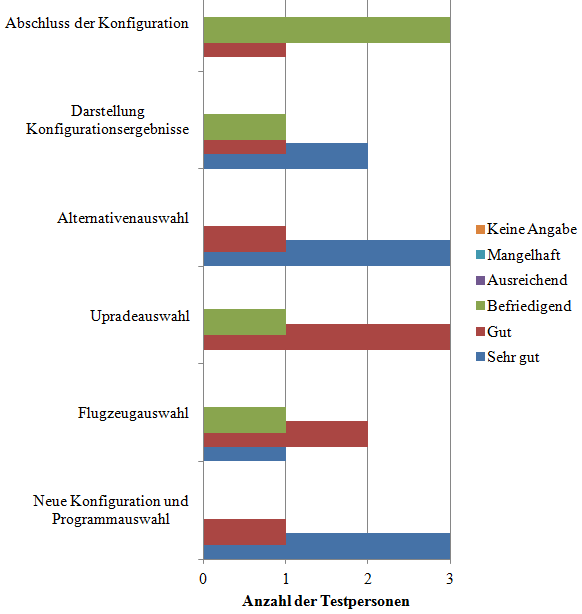
\includegraphics[width=\hsize]{images/bewertung_tablet}
\caption{Auswertung der Funktionalen Anforderungen im Fragebogen}
\label{bewertungTablet}
\end{figure}
Das Ergebnis der Fragebögen in Bezug auf die funktionalen Anforderungen ist in Abbildung \ref{bewertungTablet} zu sehen. Auffällig ist die besonders gute Bewertung für die Auswahl einer neuen Konfiguration und der Alternativenauswahl. Diese beiden Ansichten und deren Funktionen konnten während des Tests schnell gefunden, verstanden und verwendet werden. Die drei Hauptfunktionen Flugzeugauswahl, Upgradeauswahl und Darstellung der Konfigurationsergebnisse sind durchschnittlich als Gut bewertet worden. Für eine optimale Verwendung dieser Funktionen hat das Wissen eines Kunden gefehlt, der seine eigenen Flugzeuge kennt sowie eine grobe Zuordnung der Upgrades in die einzelnen Bereiche vornehmen kann. \par

Das Problem mit dem Abschluss der Konfiguration, welches sich bereits bei den Fragen der Anwendern herausgestellt hat, ist auch in der Bewertung ersichtlich. Drei der vier Anwender haben dem Abschluss der Konfiguration mit befriedigend bewertet. An dieser Stelle sollte eine Verbesserung für die Erfüllung der Anforderungen stattfinden. \par 
\begin{figure}[H]
\centering
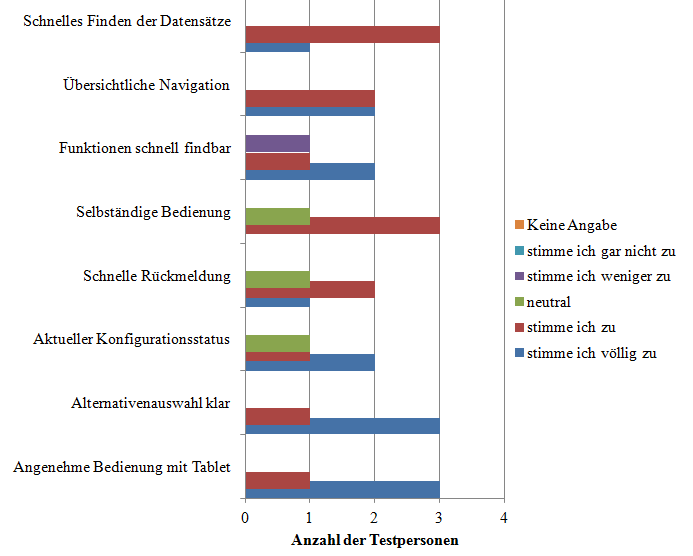
\includegraphics{images/bewertung_tabletComplete}
\caption{Ergebnisse der Usability Fragen zu der Tablet Anwendung}
\label{bewertungUx}
\end{figure}
Die Bewertungen des zweiten Teils der Evaluation sind in der Grafik \ref{bewertungUx} zu sehen. Besonders positiv fallen die Ergebnisse für die Bedienung mit dem Tablet sowie die Verständlichkeit der Alternativenauswahl auf. Es gelang damit ein Verständnis für die Auswahl von Alternativen zu schaffen, was dabei helfen sollte den Konfigurationsprozess mit dem Kunden gemeinsam durchzuführen. Diese Tatsache unterstützt die gute Bewertung beim Punkt selbständige Bedienung. Die Maßnahmen für ein flexibles und tolerantes Navigationskonzept sind im Kriterium übersichtliche Navigation sehr gut bewertet worden.

Das Ergebnis der guten Bedienbarkeit auf dem Tablet resultiert auf der ausgewählten Plattform sowie den verwendeten Bedienelementen in der Entwurfsphase. Bei der Implementierung wurde der Entwurf sehr gut umgesetzt, wodurch die gute Bewertung erklärt werden kann. \par 

Bei der ersten Verwendung der Anwendung reagiert die App langsamer als beim zweiten Mal. Der Grund hierfür ist, dass beim initialen Start die Daten erst in den Hauptspeicher geladen werden müssen. Bei der nächsten Verwendung sind diese bereits im Speicher enthalten. Da eine Verzögerung nur bei wenigen Ansichten, wie der Navigation von der Upgradeauswahl in die Zusammenfassung auftritt, ist dieses Problem aufgrund der ansonsten positiven Bewertungen bei dem Kriterium der schnellen Rückmeldung zu vernachlässigen. Zur Lösung dieses Problems sollten die Daten vorgeladen werden und in der Wartezeit ein Ladebalken angezeigt werden. Eine andere Situation liegt bei der Bewertung für die Darstellung des aktuellen Konfigurationsstatus vor. Dieser Punkt ist für die Anwendung essentiell, da der Benutzer zu jeder Zeit wissen muss, in welchem Status er sich befindet. Da auch hier die anderen Bewertungen positiv waren, ist keine eindeutige Ursache des Problems auszumachen.

\subsection{Auswertung der Expertenergebnisse}
Bei den Experten sind die Fragen gezielt nach den nicht-funktionalen Anforderungen gestellt worden. Hierbei wurden die zehn Heuristiken von Nielsen als Grundlage verwendet und jeder dieser Punkte sollte bewertet werden. Die Befragung hat die Stärken und Schwächen der Anwendung aufgezeigt. In Abbildung \ref ist das Ergebnis der Auswertung zu sehen. Für die Flexibilität der Nutzung wurde der Expertenmodus (siehe \ref{expertDesign}) entworfen. Das Ziel des Modus wurde, wie die positive Bewertung zeigt, eindeutig erreicht. Eine klare Umsetzung der Designvorgaben ist durch die gute Bewertung von Konsistenz und Standards sowie des ästhetischen und minimalistischen Designs gegeben. \par 
\begin{figure}[H]
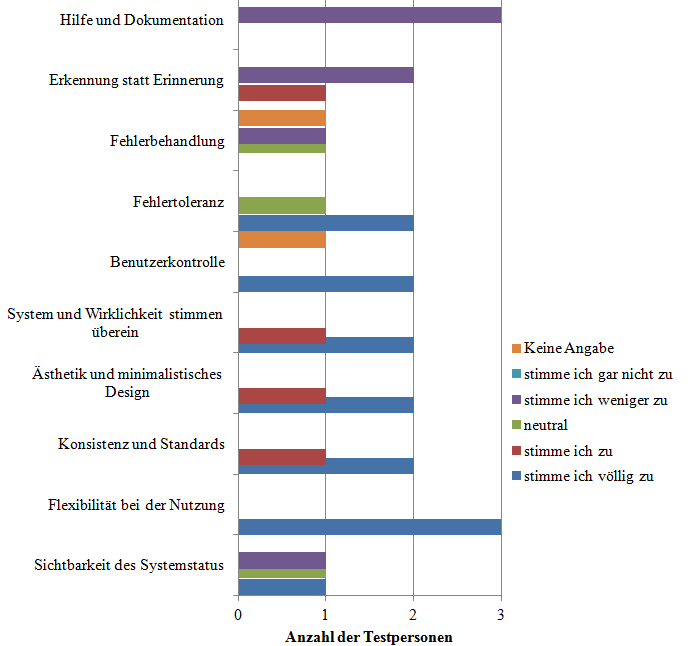
\includegraphics{images/bewertung_expert_complete}
\caption{Auszug aus der Expertenbefragung}
\label{bewertungExpert}
\end{figure}
Die Heuristiken Hilfe und Dokumentation sowie Fehlerbehandlung sind weniger gut bewertet worden, da der Fokus der Nicht-Funktionalen Anforderungen auf anderen Kriterien lag. Diese Punkte sind außerdem weniger relevant, da ein Mitarbeiter des Herstellers bei der Anwendung der App dabei ist. Die Punkte Fehlertoleranz, Benutzerkontrolle und System stimmt mit der Wirklichkeit überein erhalten ebenfalls eine gute Bewertung, obwohl diese nicht im Vordergrund standen. Dies zeigt ein positives Gesamtbild der Anwendung. \par 
Auch bei den Experten ist die dauerhafte Sichtbarkeit des Systemstatus, der analog zum Konfigurationsstatus aus den Benutzertests zu sehen ist, weniger vorhanden. Der Punkt Erkennung statt Erinnerung ist mit dieser Bewertung verwandt und erhält deshalb eine schlechtere Bewertung.  An dieser Stelle fehlt ein Leitfaden in der Anwendung, so dass die folgenden Schritte deutlicher werden. 

\section{Konsequenzen aus der Evaluation}
Die Ergebnisse der Evaluation haben zwei Probleme der Anwendung aufgeworfen. Zum einen ist der Abschluss des Auswahlprozesses, zum anderen ist der aktuelle Status der Konfiguration bzw. des Systems nicht sichtbar. Beide Problemstellen beziehen sich auf die Seite der Zusammenfassung. Diese ist als Orientierungshilfe für den Anwender konzipiert worden. Aus diesem Grund muss in dieser Ansicht der aktuelle Systemstatus und der Abschluss der Konfiguration aufgenommen werden.  
\begin{figure}[H]
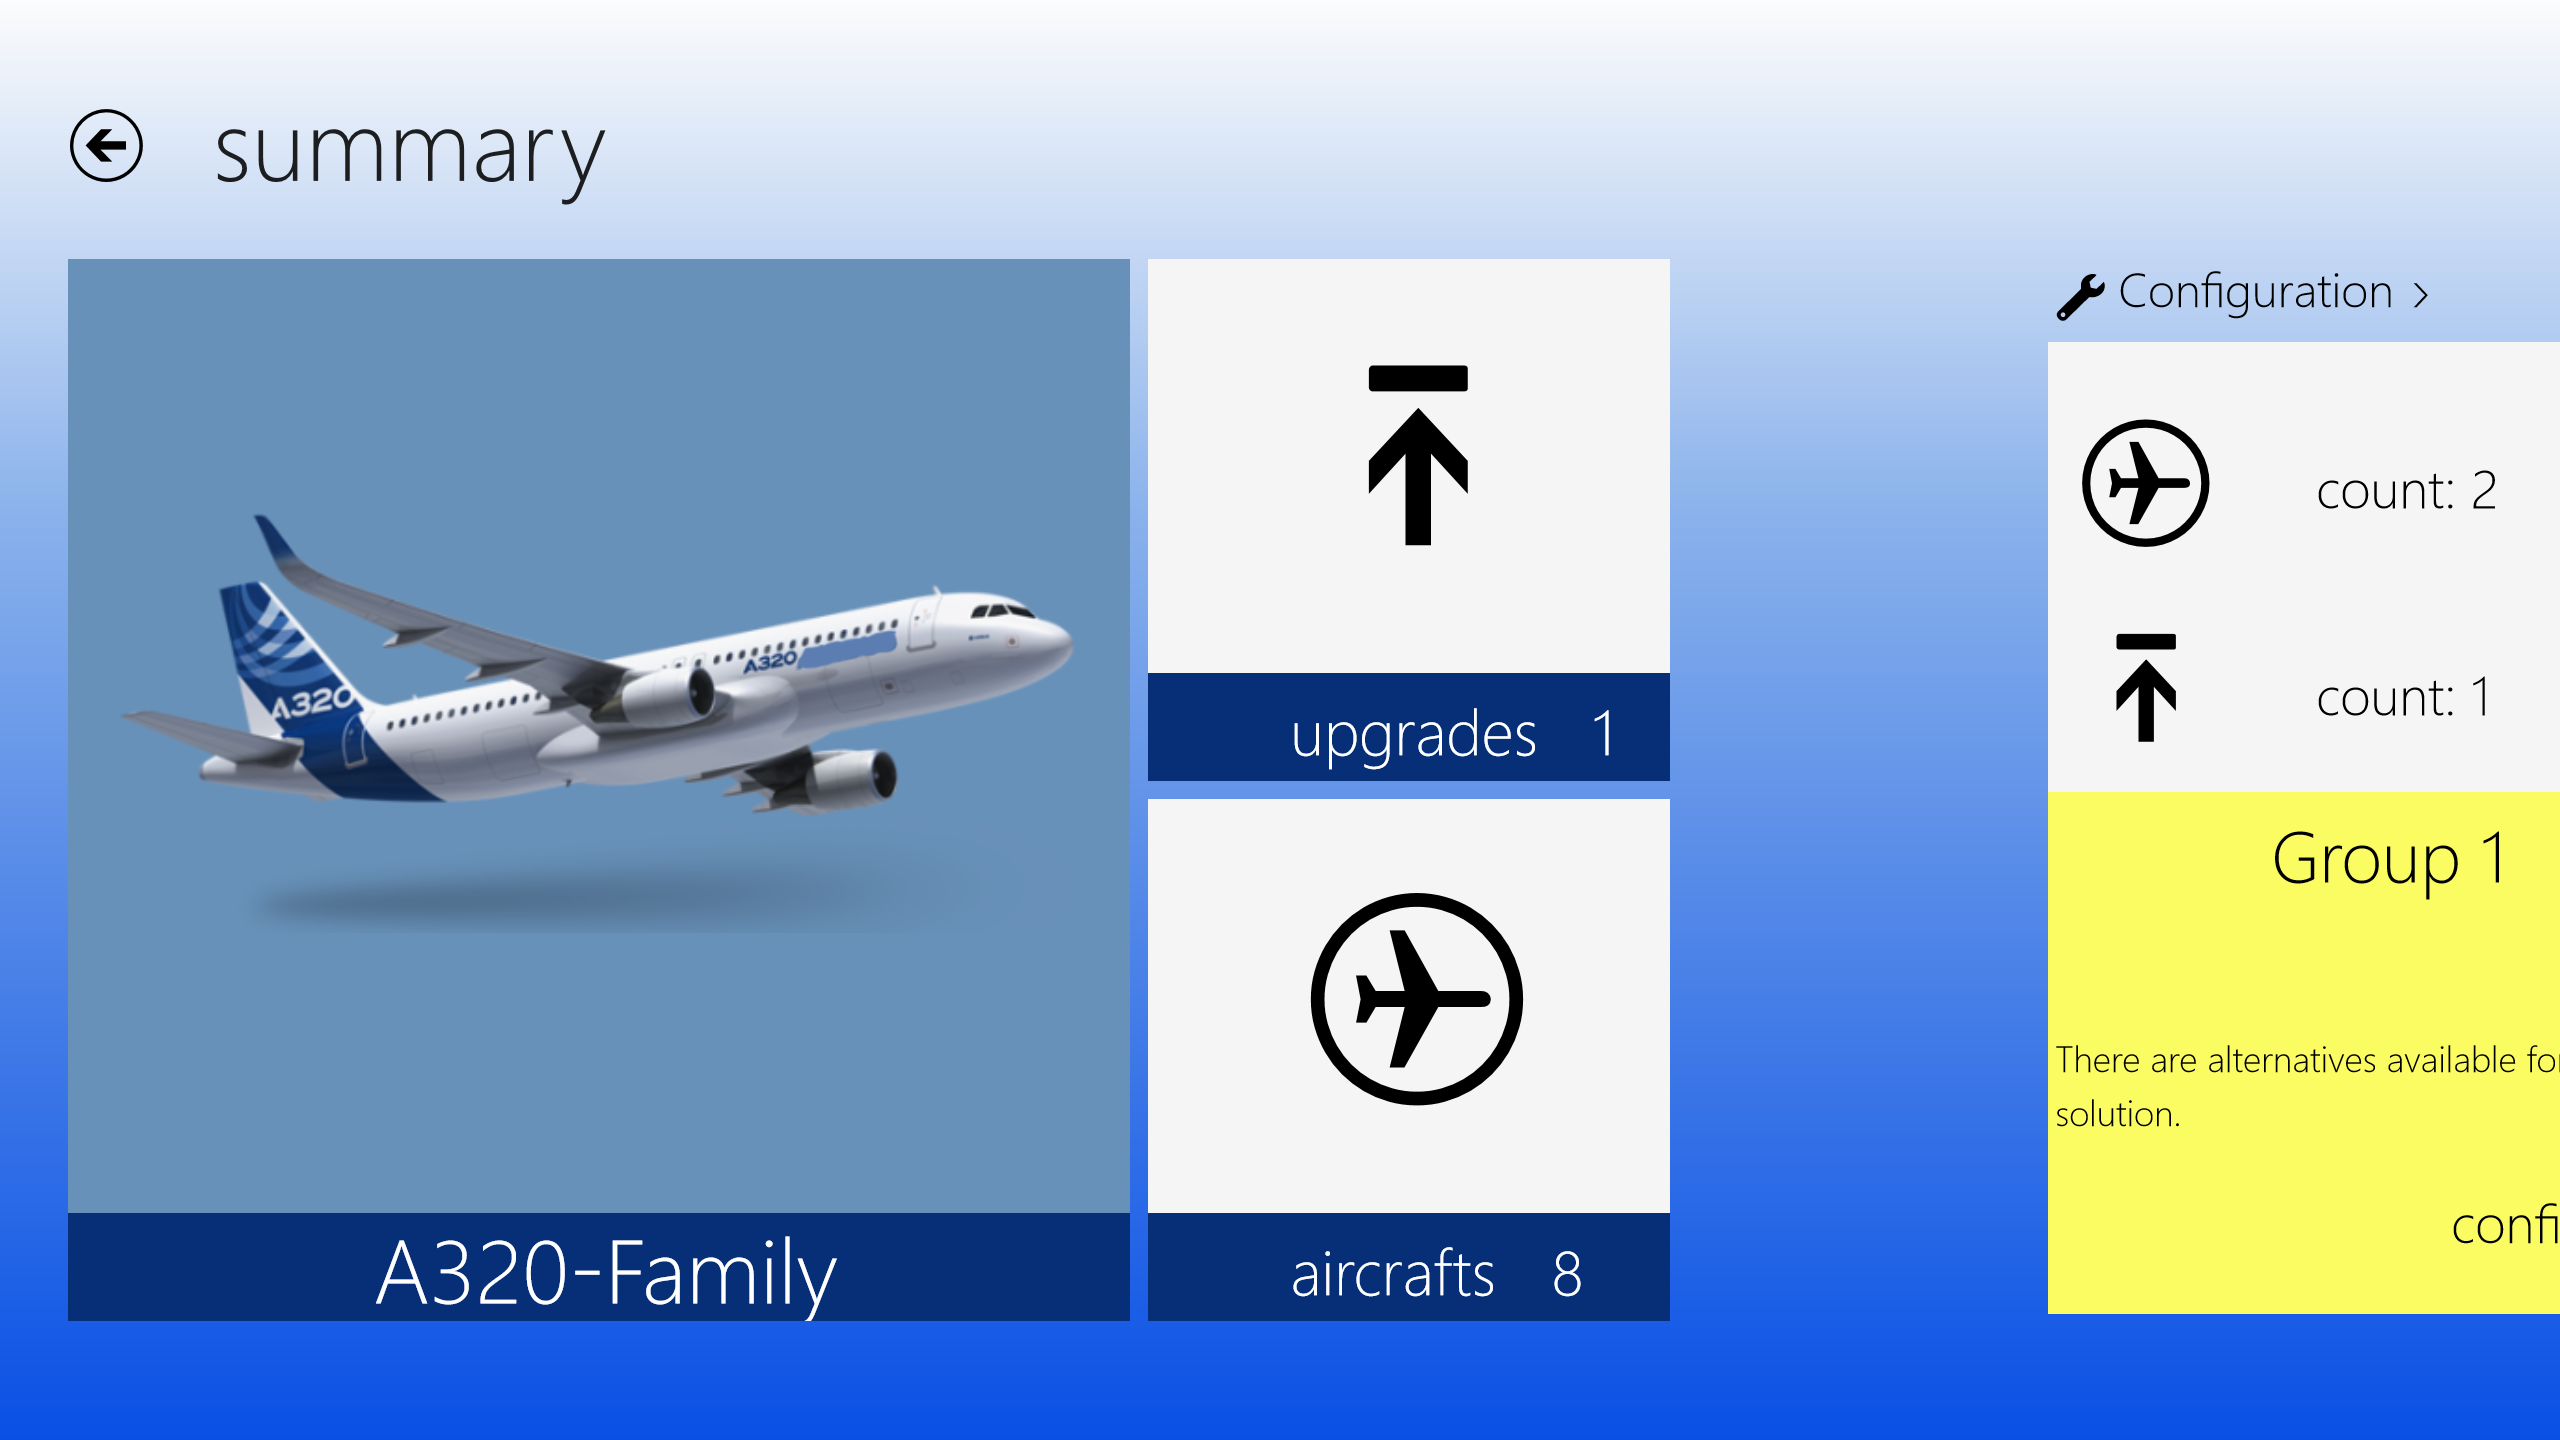
\includegraphics[width=\hsize]{images/impl/summary_impl}
\caption{Neue Zusammenfassungsansicht, nach dem Redesign}
\label{redesignSummary}
\end{figure}
Abbildung \ref{redesignSummary} zeigt den neuen Entwurf der Zusammenfassung. Die Idee ist der Mathematik entnommen, bei der Eingabe A + Eingabe B = Ergebnis C ergibt. Angewendet auf die Ansicht bedeutet dies, dass zuerst die Eingabedaten Flugzeug und Upgrades angezeigt werden und als Resultat die Konfigurationsgruppen gebildet werden. Weiterhin wird die Navigation zur Flugzeug- und Upgradeauswahl mit einer Kachel durchgeführt. Für eine bessere Übersicht erhalten die Kacheln die Anzahl der ausgewählten Elemente. Dies verhindert ein zu langes Scrollen bei größeren Selektionen. 
Der Abschluss der Konfiguration wird durch ein dauerhaftes Anzeigen der AppBar verbessert. Hierdurch sind die Buttons für einen Abschluss der Konfiguration dauerhaft sichtbar.\par 

Für eine zukünftige Entwicklung der App sind die weiteren Heuristiken interessant. Diese waren im Evaluationsbogen der Experten, jedoch nicht in der Zielsetzung der Anforderungen enthalten. Aufgrund der unterschiedlichen Bewertung der Experten in diesen Kriterien können hier weitere Verbesserungen durch die Umsetzung der Punkte erzielt werden. \par 